\chapter{Theoretical Background}\label{ch:theory}

\section{State-Of-The-Art}\label{sec:state_art}

\subsection{Sampled sounds vs Procedural audio}

Sampled sound is still the most typical technique for digital audio in the game industry since its sophistication in the late 1990s when game music moved to recorded tracks on CD. Present game audio systems can compare to professional samplers on account of the improvement of hardware decompression and compressed audio formats \cite{farnell2007introduction}. But this method has limitations due to its static and repetitive nature which does not allow to model the sound of an object based on its physical interactions in a game scene. This leads to inconsistencies between the visuals and their associated soundtrack \cite{picard2009expressive}. Despite the use of different processes such as filtering, pitch-shifting and time-scaling to name but three, sampled sounds can not compare to the versatility that procedural audio offers. With the increasing interest that the game industry has put into \gls{VR} and \gls{AR}, it is becoming essential to provide realistic and compelling sounds in these virtual environments to provide immersion and presence to the user. An obvious advantage of procedural audio over recordings is the large memory storage space that is necessary due to the huge amount of audio assets present in modern games. The ability of procedural audio to generate sounds automatically based on the interactions of the objects in a scene eases the asset management task for the audio team. Instead, the sound designer becomes more of a programmer by taking into account the object’s behaviour and physical properties to create sounds. This does not mean that the sound designer is replaced by procedural content as certain tasks need special attention to deliver high quality sounds. Regardless of its advantages, procedural audio still lacks of development tool chains and presents conflicts with current methods due to its still scarce use in the industry \cite{farnell2010designing}.

\subsection{Sound synthesis in virtual and interactive applications}

Researchers have been working on automatically generated synthesized sounds based on physical interactions for quite some time now. Different publications that have contributed to the creation of procedural sounds in virtual environments and that have inspired this thesis are discussed in this section.

In \cite{gaver1993we, gaver1993world} Gaver proposes the analysis and synthesis of contact sounds based on what he calls "every listening" which consists in focusing on the perceptual features of a sound event. Another pioneering work \cite{takala1992sound} presents a methodology to produce synchronized sounds with animations. Later, in \cite{doel1998sound} the author focuses on the computation of "natural" sounds produced by physical objects in VR. A finite element based simulation method is used in \cite{director2001synthesizing} that takes advantage of existing simulation techniques already used for physically based animation although it is expensive and non-interactive. In his book \cite{Cook:2002:RSS:515316}, Cook covers extensively physically based sound synthesis concepts and defines a parametric model as one that can be manipulated to change the interaction, object and sound.  Other works have acquired a modal model of objects with arbitrary shapes through modal analysis \cite{james2006precomputed, raghuvanshi2006interactive} and controlling modal synthesis by game engine collision events.

\cite{van2001foleyautomatic} and \cite{lloyd2011sound} make use of modal models derived from recordings of struck objects which is similar to the approach described in this thesis. This model is used to create impact, rolling and sliding sounds.

\textit{Wildes and Richards (1988)} defined the angle of internal friction ($\phi$), a shape-invariant acoustical parameter that heuristically categorizes sounds into material categories, as
\begin{equation}\label{eq:tanf}
\tan(\phi) = \alpha / \pi f,
\end{equation}
where $\alpha = \tau_e$ is the damping coefficient, with $\tau_e$ being the time for the vibration amplitude to decay to $1/e$ of its original value after the object is struck  and $f$ is the vibration frequency\cite{giordano2006material}.

\begin{itemize}
\item (Precomputed Acoustic Transfer: Output-sensitive, accurate sound generation for geometrically complex vibration sources) has a good related work chapter
\item  Florens and Cadoz (The physical model: modeling and simulating the instrumental universe): the first to introduce modeling of surface vibrations with physical models
\item Van den Doel (Scanning physical interaction behavior of 3D objects): robotic device to measure impulse response of an object being struck in different points
\item  O`Brien et al (Synthesizing Sounds from Rigid-Body Simulations): FEM (very accurate cause its based on physically measured data but very complicated to extract and require too much processing power)
\item D. L. James, J. Barbic, and D. K. Pai (Precomputed Acoustic Transfer: Output-sensitive, accurate sound generation for geometrically complex vibration sources): BEM
\item Raghuvanshi and Lin (Interactive sound synthesis for large-scale environments.): spring-mass system approximation
\item Ren,Yeh,Lin (Example-Guided Physically Based Modal Sound Synthesis): one simple recording
\item PHYSIS project: PHYsically informed and Semantically controllable
Interactive Sound synthesis
\item Van del Doel (FoleyAutomatic: physically-based sound effects for interactive simulation and animation): modal models derived from sound samples
\item Brandon Lloyd et al. (Sound Synthesis for Impact Sounds in Video Games): short-time Fourier Transform
\item Perry Coook (Real Sound Synthesis for Interactive Applications): a review of the work done on this field (physically-based synthesis in computer music).
\end{itemize}
\Todo{turn the bullets into text}


This thesis adopted the parameter extraction from recordings. We used everyday objects, making it easy for us to record sounds and model them on the computer. We also chose this method to make it easy for users of our product to extend the repository of physically-based impact sounds of objects.

\section{Sound Production}

For computer sounds to be produced, force models are used as input to the sound synthesis algorithm. In other words physics is used as the excitation parameter to produce sound. \cite{van2003modal} refers to four different interaction models that produce the excitation force.

\begin{enumerate}
\item Impact force, produced during collisions,
\item Continuous contact force, produced during rolling or scratching of an object,
\item Combustion engine forces and
\item Live data streams
\end{enumerate}

This thesis examines sounds produced by the first two models. Impact forces are applied when two objects collide. They last for a short period of time and depend on the physical attributes of the objects. Constant contact forces are produced while an object is rolling on a surface of scratching/sliding on it. They can be modeled as successive impact forces, where one adds on top of the other. The distinction between roll or scratch depends on the shape of the object and on the hardness of both surfaces.

In this thesis we focus on sound produced by rigid-body objects. When two of these objects collide, the energy from the impact deforms them. This deformation is propagated through the whole object, making its outer surfaces vibrate and emit sound waves to the environment. Sound waves impact on other objects in the environment and get reflected and absorbed from them before reaching the ear \cite{van1998sounds}. All the interactions that happen before reaching the ear, contribute to the characterization of the sound, making the listener able to visualize the impact just by sound. Since in this thesis we examine only object-related interactions and not environmental ones, below we explain in depth how each of these physical attributes affect sound.

\subsection{How physical attributes affect sound}

Impact sounds consist of an excitation that dampens over time. Hence, the amplitude of the oscillation depends only on the damping. On the other hand, scraping sounds consist of continuous supply of energy that adds to the amplitude value on top of the damping of the oscillation throughout the object interaction. In addition, the force of the interaction plays the most significant role for the amplitude of the oscillation. The stronger the force, the biggest it imposes the amplitude value to be - and the louder the sound \cite{gaver1993world}.

Furthermore, the material of the interacting objects affects their vibrating oscillation. \colorbox{pink}{Damping factor is a material-specific attribute and the bigger it is, the faster the objects lose} \colorbox{pink}{energy and thus the oscillation lasts shorter. For example, wood has way bigger damping}\\ \colorbox{pink}{factor than metal and this is why they produce a ``thud'' and a ``ringy'' sound respectively. } Moreover, in \cite{klatzky2000perception} they have proven that material and spectral characteristics are correlated, for example glass is found to include in general higher frequencies than rubber. 

Moreover, the configuration of the object also affects its vibration. The size of it determines how high or low pitched sound it will produce. More specifically, the smaller the object the more high pitched will be the sound. Elasticity, on the other hand, influences the impact force since the more elastic an object the steeper the increase of the size of colliding area.  

Table \ref{tab:acoustic_effects} shows the acoustic \colorbox{pink}{information} affected by each physical attribute. 

\begin{table}[H]
	\centering
    \begin{tabular}{ | l | l |}
    \hline
    \textbf{\textit{Attribute}} & \textbf{\textit{Effects on the Sound Wave}} \\ \hline
    \multicolumn{2}{|l|}{\hspace{2.2cm} \textit{Interaction}} \\ \hline 
    \hspace{8pt} Type & Amplitude, spectrum \\ 
    \hspace{8pt} Force & Amplitude, bandwidth \\
    \hline
    \multicolumn{2}{|l|}{\hspace{2.2cm} \textit{Material}} \\ \hline
    \hspace{8pt} Density & Frequency \\
    \hspace{8pt} Damping & Amplitude, frequency \\
    \hspace{8pt} Homogeneity & Amplitude, frequency \\
    \hline
    \multicolumn{2}{|l|}{\hspace{2.2cm} \textit{Configuration}} \\ \hline
    \hspace{8pt} Shape & Frequency, spectral pattern \\ 
    \hspace{8pt} Size & Frequency, bandwidth \\
    \hspace{8pt} Elasticity & Amplitude, frequency \\
    \hline
    \end{tabular}
    \caption{Acoustic effects of source attributes \cite{gaver1993world}.}
    \label{tab:acoustic_effects}
\end{table}

\section{Modal Analysis}\label{sec:modal_analysis}
In this thesis we are using solid objects that are struck in different ways to produce sound, namely falling on the floor or colliding with another object. The sounds produced can be impact, rolling or scratching sounds. When an object is struck, the forces applied cause deformations to it, emitting sound waves through the vibration of its outer surfaces \cite{van2001foleyautomatic}.

Modal analysis studies the response of models under excitation. It uses the 3D model of an object to calculate its modal modes (vibration modes). There are multiple ways to do this, with the most accurate being \gls{FEM} (Finite Element Method). The objective of \gls{FEM} is to calculate the natural frequencies of a structure when it vibrates freely.

Another method for modal analysis is the ``Example-guided'', where data get extracted using example recordings of the objects being struck. Using a suitable algorithm it is easy to extract features from the recordings such as the fundamental frequency and its harmonics and the frequency peaks of the signal (amplitudes).

Since it is a time consuming procedure, generally it takes place in the pre-computation phase. Its results are stored and used in real-time phase.

\subsection{Data Extraction}\label{sec:data_extract}
Modal analysis is performed before modal synthesis, to extract the necessary data. Synthesis is a method of generating sound using the provided information, as it will be discussed further below. The data needed for synthesis and the ways we obtained each one of them are shown in the table \ref{tab:extracted_data}.

\begin{table}[H]
	\centering
    \begin{tabular}{ | l | l | l | p{5cm} |}
    \hline
    \textbf{Symbol} & \textbf{Description} & \textbf{Derivation} \\ \hline
    $A_n$ & Initial amplitude & Modal analysis \\ \hline
    $d_n$ & Damping & Material properties \\ \hline
    $f_n$ & Modal frequency & Modal analysis \\
    \hline
    \end{tabular}
    \caption{Derivation of data used in modal synthesis.}
    \label{tab:extracted_data}
\end{table} 

Since every different point being struck produces different deformations on the object, we need matrices to represent the data needed for each point. More specifically, we need a vector $\textbf{f}\sim (K \times 1)$  corresponding to the modal frequencies of every point, a vector $\textbf{d}\sim (K \times 1)$ corresponding to the damping ratios and a matrix $\textbf{A}\sim (K \times N)$, which corresponds to the amplitudes of each mode in every point of the object, where $K$ is the number of modal frequencies calculated in one point and $N$ the number of points. All the above gives the modal model which can be symbolized as $\textbf{M} = \{\textbf{f}, \textbf{d}, \textbf{A}\}$ \cite{van2001foleyautomatic}.
 
\section{Modal Synthesis}\label{sec:modal_synth}
Modal synthesis is the sum of damped oscillators each corresponding to a modal frequency. In this part, using the data extracted above, we synthesize the struck sound corresponding to the object. When an object is struck, a sound envelope (Attack Decay Sustain Release, \textbf{ADSR}) is produced. Attack is the onset of the signal and is the most influential to the characteristic sound of the object. Some of the frequencies exhibit a fast decay, while others are sustained more.  Finally at the release phase the sound stops. There are different ways to synthesize impact sounds, two of them being ``Sinusoidal Additive Synthesis'' and ``Filter-based Modal Synthesis''. The former uses exponential damping and the latter band-pass filters where the damping is the Q-factor of the filter. 

\subsection{Sinusoidal Additive Synthesis}\label{sec:sin_synth}

This method is based on Fourier theory which states that any sound can be expressed mathematically as a sum of sinusoids. The term ``additive'' refers to sound that is generated by adding together the output of multiple sine wave generators which are modulated by amplitude and frequency envelopes \cite{smith2011spectral}.

The frequencies used for sound synthesis are the ones at which an object vibrates when struck and are called \textit{resonant modes}. On excitation, the sine waves representing the mode vibrations peak to the designated amplitude and then start decaying over time. High frequency modes decay faster than low frequency ones \cite{lloyd2011sound}, leaving a low-pitched residue named \textit{``tail''}, especially when damping is low.

\cite{Cook:2002:RSS:515316} points out that the vibrational modes of a  metal plate can be predicted by the shape and the location of the impact on the object, which leads to recognize the power of a sound synthesis model based on the sum of several sinusoidal modes. Figure \ref{fig:sin_add_synth} shows a model that enables to control the amplitudes and frequencies of a bank of sinusoidal oscillators.

\begin{figure}[H]
  \centering
    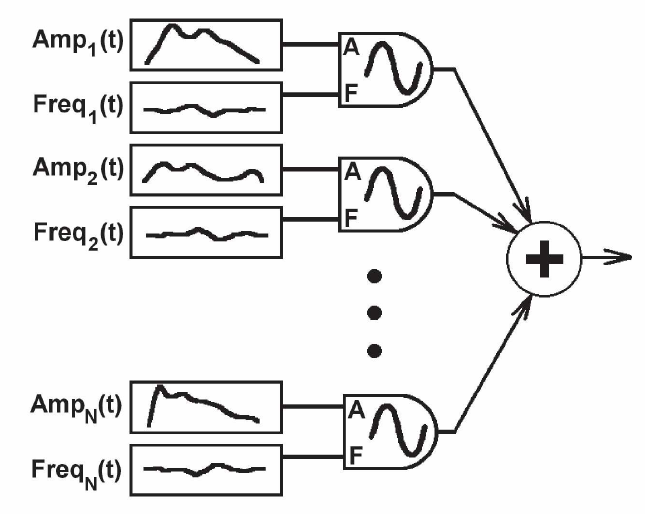
\includegraphics[width=0.5\textwidth]{sinusoidal_add_synth.PNG}
      \caption{Sinusoidal Additive Synthesis Algorithm \cite{Cook:2002:RSS:515316}.}
      \label{fig:sin_add_synth}
\end{figure}

Mathematically, at a struck point $k$ when vibrating in mode $n$, the impulse response of the model is:
\begin{equation}\label{eq:modal_response}
y_k(t) = \sum\limits_{n=1}^{N} A_{nk}\ e^{-d_n t}\ \cos(2 \pi f_nt)
\end{equation}
if $t\leqslant 0$ and $y_k = 0$ if $t<0$ \cite{van2001foleyautomatic}. The decay rate $d_n$ of each mode is object-dependent, it determines the energy loss due to the vibration and is related to the material of the object. The amplitudes $A_n$ and the frequencies $f_n$ are the resonant data extracted during the modal analysis. Modal frequencies are a set of frequencies that determine the object and remain the same, while amplitudes are vertex-specific and change depending on the excitation point.

\subsection{Filter-based Modal Synthesis}\label{sec:add_synth}

\paragraph{Band-pass Filters\\}\label{par:bpf}

At this point we will give some basic description of the band-pass filter since it is widely used in this thesis. Band-pass filters (\gls{BPF}s) take a signal as input and let only a range of frequencies to pass while attenuating the rest. This range depends on the central frequency $f_c$ and the bandwidth. A filter of this kind is a result of a cascading of a low-pass and a high-pass filter circuit.

\textbf{Bandwidth (BW)} is the passing range or ``band'' of frequencies. Defining as 0db the resonant peak, we can find the two cut-off frequencies ($f_{c,low}$ and $f_{c,high}$) at -3dB. The difference between those two is the bandwidth  
\begin{equation}\label{eq:bw}
BW = f_{c,high}-f_{c,low}.
\end{equation}   
In figure \ref{fig:resp_bpf} we can see the frequency response of a BPF \cite{bib:bpf}. 

\begin{figure}[H]
  \centering
    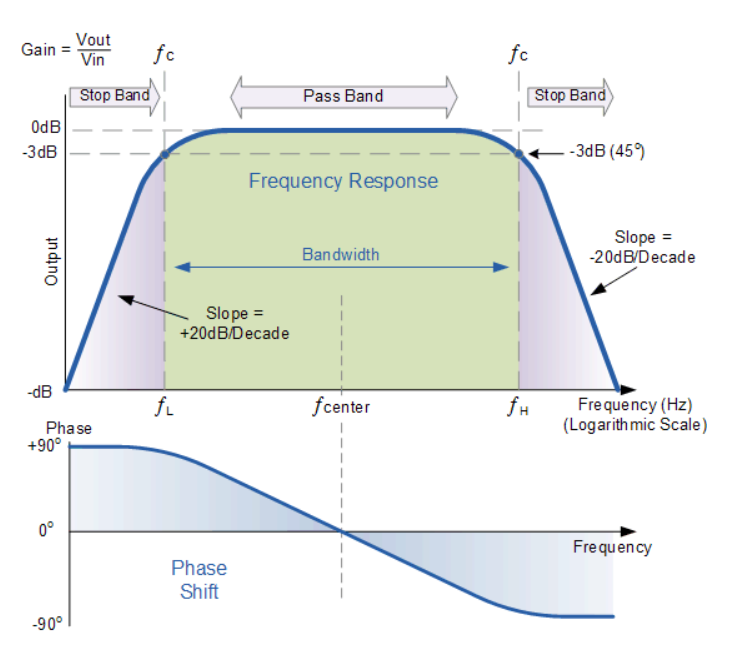
\includegraphics[width=0.7\textwidth]{BPF.PNG}
      \caption{Frequency Response of a Band-pass Filter  \cite{bib:bpf}.}
      \label{fig:resp_bpf}
\end{figure}

\paragraph{Modal Synthesis\\}\label{par:synth}

This method is also additive, since we are adding the outputs of a number of band-pass filters. To synthesize a sound using this method, we use as many filters as the modal frequencies. A filter is constructed using modal frequencies of the object as center frequencies and the damping of the material is used to control the \textbf{Quality factor (Q)} of the filter.  The Q-factor is calculated heuristically, depending on the material of the sound and is inversely proportional to the bandwidth ($Q=f_c/BW$), so the lower the Q-factor, the wider the bandwidth and vice-versa. Using amplitudes from matrix \textbf{A} (section \ref{sec:data_extract}), the level of the passing frequencies is controlled and resonators can be created through these filters. 

\begin{figure}[H]
  \centering
    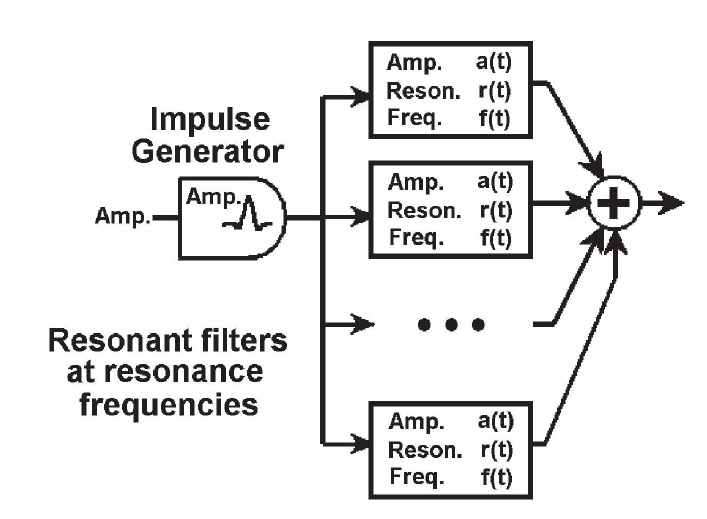
\includegraphics[width=0.5\textwidth]{filter-based_add_synth.PNG}
      \caption{Filter-based Modal Synthesis Algorithm \cite{Cook:2002:RSS:515316}.}
      \label{fig:filter_synth}
\end{figure}

\subsection{Sound Variations} \label{sec:sound_variation}
Each point of an object produces a different sound when struck. This happens because of the different amount of excitation each resonant mode experiences. As mentioned above, during data extraction we get a matrix of amplitudes of size $K\times N$ corresponding to $K$ different resonant modes of each of the $N$ points of the object. This means that even though resonant frequencies are the same for each location of the specified object, each frequency's peak differentiated depending on the location.

There are several methods to achieve spatial variation on sound produced from the same object. 
\begin{itemize}
\item The most accurate method is to perform FEM analysis on the object and distill as many amplitude matrices as the number of points consisting it. However, this method needs a lot of memory to store the data and computational power to access them. This method is used in \cite{o2002synthesizing}.
\item Another less precise method is to separate the object into areas and assume that each point belonging in the same area will sound exactly the same. Thus, the amount of stored data decreases in a great deal while at the same time the sounding result is almost the same.
\item A third method is to store only one amplitude matrix and randomize the values for each impact sound, but this can lead to sounds inconsistent with the collision location. This method is used in \cite{lloyd2011sound}.
\item Finally, a better approach to the previous method is to retain the same amplitude values for all points of the object, but apply a texture map on the object which indicates changes on the pitch of the sound all over the object. For instance, the near-edge points of an object produce a higher-pitched sound than the ones in the center of each faces. 
\end{itemize}

\section{3D Audio}
In VR/AR applications, the location of the incoming sound plays as significant role as the sound itself. 

\Todo{explain HRTF}